% ECE 285 HW1 draft. Compile here with pdflatex report.tex twice.
% Replace the author name before submission. Only completed runs are reported.
\documentclass{article}
\usepackage[preprint,nonatbib]{neurips_2024}
\usepackage[T1]{fontenc}
\usepackage[utf8]{inputenc}
\usepackage{amsmath,amssymb,graphicx,booktabs}
\usepackage[hidelinks]{hyperref}
\usepackage{url}
\makeatletter
\renewcommand{\@noticestring}{ECE 285: Homework 1. Draft report.}
\makeatother
\title{Generating Chest X-rays with a VAE}
\author{Your Name\\ECE 285: Homework 1, UC San Diego}
\begin{document}
\maketitle

\section{Method}
We implement a convolutional VAE~\cite{vae} in PyTorch. The encoder predicts a diagonal Gaussian
$q_\phi(z\mid x)$ through mean $\mu$ and log variance $\ell$.
We sample $z=\mu+\exp(\ell/2)\odot\epsilon$, where
$\epsilon\sim\mathcal{N}(0,I)$, and minimize
\begin{equation}
\mathcal{L}=\frac1B\sum_{i=1}^B\left[
\sum_p(x_{ip}-\hat{x}_{ip})^2+
\frac\beta2\sum_j(\mu_{ij}^2+e^{\ell_{ij}}-1-\ell_{ij})\right].
\end{equation}
Terms are summed per image and batch-averaged. Squared error is a Gaussian
likelihood loss (variance $1/2$); $\beta=1$ gives the negative ELBO up to a constant.

Encoder blocks use kernel 4, stride 2, padding 1, LeakyReLU(0.2), and channels
$(16,32,64,128)$ by default. Linear posterior heads and a mirrored transposed-CNN
decoder with ReLU/final sigmoid complete the model. Generation decodes prior draws into image means.

\section{Experimental setup}
Kaggle X-rays~\cite{dataset} are split into 5,216 training, 16 validation, and 624
test images, pooling classes without labels. Inputs are grayscale, square-resized,
scaled to $[0,1]$, without augmentation. CPU training uses Adam, learning rate
$10^{-3}$, batch size 32, and 30 epochs ($64^2$ baseline) or 40 (others).
Checkpoints minimize validation loss. Training seeds are listed in Table~\ref{tab:results}.

\paragraph{Evaluation.}
Following Ignite~\cite{ignite}, 624 prior samples (seed 123) and 624 test images
are evaluated in batches of 16. Real originals and native generated outputs
are resized to $299^2$. Inputs use PIL bilinear resizing, uint8/RGB conversion,
and $[0,1]$ scaling. Frozen Inception v3 retains \texttt{transform\_input=True}, without
external normalization. FID uses \emph{1,000 softmax probabilities}, not 2,048
pooled features; benchmark scales differ. IS uses the full generated set.
All reported runs share the fixed real reference.

\begin{figure}[!h]
\centering
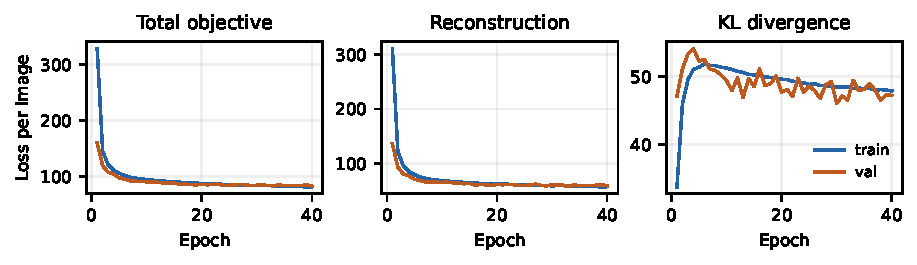
\includegraphics[width=.95\linewidth]{figures/training_curves.pdf}
\caption{Training and validation losses: three blocks, $128^2$, latent 32,
$\beta=0.5$, seed 42. Losses decrease, with noisy validation estimates.}
\label{fig:curves}
\end{figure}

\clearpage
\section{Results and discussion}
Table~\ref{tab:results} reports selected checkpoints. MSE divides validation
reconstruction sums by pixel count; cross-resolution targets still differ.

\begin{table}[h]
\centering
\caption{$H$: image side; $D$: blocks; $d_z$: latent dimension; $s$: training
seed; $e^*$: selected epoch. MSE is validation pixel MSE. Lower FID and higher IS
are conventionally preferred.}
\label{tab:results}
\small
\begin{tabular}{rrrrrrrrr}
\toprule
$H$ & $D$ & $d_z$ & $\beta$ & $s$ & $e^*$ & MSE & FID & IS\\
\midrule
64  & 4 & 32 & 1  & 42 & 23 & .006006 & .2351 & 1.4971\\
128 & 4 & 32 & 1  & 42 & 38 & .004090 & .2462 & 1.8396\\
128 & 4 & 64 & 1  & 42 & 38 & .004163 & .2459 & 1.8723\\
128 & 4 & 32 & .5 & 42 & 32 & .003562 & .2440 & 1.9334\\
128 & 4 & 32 & 2  & 42 & 38 & .004997 & .2518 & 1.7648\\
128 & 4 & 32 & .5 & 43 & 40 & .003586 & .2334 & 1.9352\\
128 & 4 & 32 & 1  & 43 & 33 & .004195 & .2766 & 1.9183\\
128 & 3 & 32 & .5 & 42 & 40 & .003628 & \textbf{.2150} & 1.9546\\
128 & 5 & 32 & .5 & 42 & 28 & .003598 & .2785 & \textbf{1.9675}\\
\bottomrule
\end{tabular}
\end{table}

\paragraph{Resolution, latent size, and regularization.}
Increasing resolution does not consistently improve FID, and doubling latent
dimension gives negligible benefit. Lowering $\beta$ from 1 to 0.5 reduces pixel
MSE by 13--15\% and improves FID/IS in both seeds. At seed 42, KL increases from
32.54 to 46.20, reflecting weaker regularization. $\beta=2$ worsens reconstruction
and both generation scores. Total losses across beta values are different objectives.

\paragraph{Architecture.}
Three blocks lower FID by approximately 12\% versus four blocks, despite slightly
worse reconstruction. Five blocks have the highest IS but worse FID.
Depths 3/4/5 yield $16^2/8^2/4^2$ final feature maps and 1.672/1.140/1.791M
parameters at $128^2$; this is not an isolated depth effect.

\begin{figure}[h]
\centering
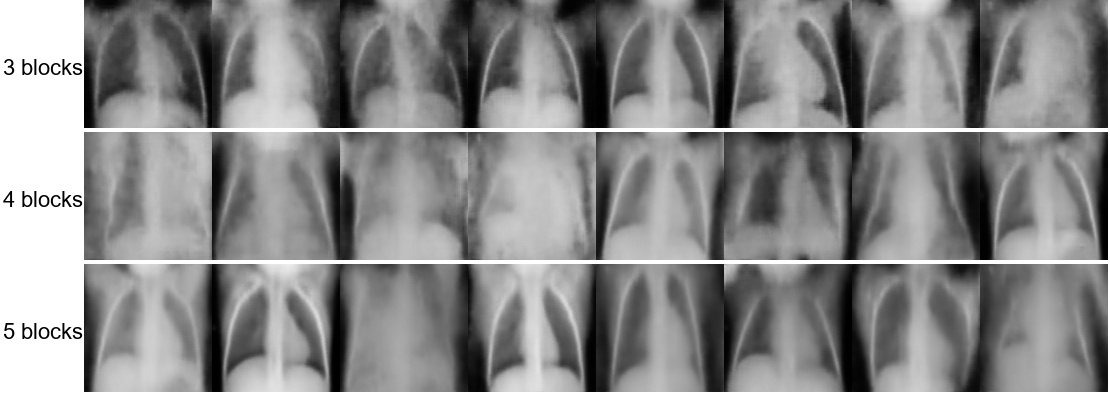
\includegraphics[width=.88\linewidth]{figures/depth_samples.png}
\caption{First eight evaluated prior draws, generation seed 123. Rows: 3/4/5
blocks; all use $128^2$, latent 32, $\beta=0.5$, training seed 42. Selected epochs:
40/32/28. Broad chest shapes vary, but detail remains blurred or patterned.}
\label{fig:samples}
\end{figure}

\paragraph{Limitations and conclusion.}
Validation has only 16 images; test metrics were inspected during exploration,
so these are descriptive results, not an untouched holdout assessment. Two seeds
support the beta comparison; depth uses one. Resolution also changes budget,
capacity, and reconstruction/KL balance. Small sample counts and ImageNet features
limit metric interpretation. $\beta=0.5$ is promising; the three-block FID advantage
needs seed replication and parameter-matched testing. Clinical validity is not established.

\begin{thebibliography}{3}
\small
\bibitem{vae} D.~P. Kingma and M. Welling. Auto-Encoding Variational Bayes.
ICLR, 2014. \href{https://arxiv.org/abs/1312.6114}{arXiv:1312.6114}.
\bibitem{dataset} P. Mooney. Chest X-Ray Images (Pneumonia).
\href{https://www.kaggle.com/datasets/paultimothymooney/chest-xray-pneumonia}{Kaggle dataset}.
\bibitem{ignite} PyTorch-Ignite. GAN evaluation using FID and IS.
\href{https://pytorch-ignite.ai/blog/gan-evaluation-with-fid-and-is/}{Evaluation tutorial}.
\end{thebibliography}
\end{document}

